%%%%%%%%%%%%%%%%%%%%%%%%%%%%%%%%%%%%%%%%%%%%%%%%%%%%%%%%%%%%%%%%%%
\section{Verification against exact solutions}\label{sec:verification_exact}
%%%%%%%%%%%%%%%%%%%%%%%%%%%%%%%%%%%%%%%%%%%%%%%%%%%%%%%%%%%%%%%%%%
% Results-section skeleton (October 2026): structure, set-ups, measured
% quantities and planned figures/tables only. Every number marked \tbd comes
% from the computational campaign (campaign/HANDOFF.md, streams R1-R7) run
% from the tagged solids4foam release; nothing in Sections 4-9 is to be
% filled from results recorded before that tag (audit A1,
% paper-data/a1_monolithic_study_inventory.md).
% Stream feeding this section: R1.

Sections~\ref{sec:verification_exact} to~\ref{sec:limitations} assess the method on the cases summarised in Table~\ref{tab:case_overview}, under the common protocol of Section~\ref{sec:protocol}.
This section verifies the method against two exact solutions and uses them to examine the interface treatment of Section~\ref{sec:numerical_methods}.

\begin{table}[htbp]
	\centering
	\small
	\setlength{\tabcolsep}{4pt}
	\caption{Cases, the questions they address in this paper and the reference used for each. Full set-ups and the provenance of the references are given in the companion verification paper~\protect\citetodo{companion verification paper}.}
	\label{tab:case_overview}
	\begin{tabular}{llll}
		\toprule
		Case & Section & Question & Reference \\
		\midrule
		ringAddedMass & \ref{sec:ring_m}, \ref{sec:interface_comparison}, \ref{sec:robustness_ring} & added mass, interface treatment, robustness & exact \\
		womersleyTube & \ref{sec:womersley_m}, \ref{sec:womersley_consistency} & viscous traction on a deforming wall & exact \\
		cavityFlexibleBottom & \ref{sec:cavity_m}, \ref{sec:robustness_cavity} & consistency with partitioned coupling & partitioned, same meshes \\
		collapsibleChannel & \ref{sec:robustness_collapsible} & robustness, massless wall & oomph-lib \\
		Hron--Turek FSI3 & \ref{sec:fsi3_m} & work--precision & Featflow \\
		blobInTreacle & \ref{sec:blob_m} & temporal accuracy & self-convergence \\
		3dTube & \ref{sec:scaling_3d} & parallel scaling, preconditioner & partitioned, same levels \\
		foilInWind & \ref{sec:lim_foil} & time-step limit & partitioned \\
		\bottomrule
	\end{tabular}
\end{table}
% Decision (Philip, 31 Oct 2026): unused monolithic variants go to Appendix app:additional_cases for now.
The remaining solids4foam tutorials with a quasi-monolithic variant (beamInCrossFlow, perpendicularFlap, membraneRoof, mokLidDrivenCavity and Hron--Turek FSI1) are not needed for this assessment and are listed in Appendix~\ref{app:additional_cases}.

%%--------------------------------------------------------------------------------------------------------------------%%
\subsection{Assessment protocol}\label{sec:protocol}
%%--------------------------------------------------------------------------------------------------------------------%%
% Source of the protocol: campaign/HANDOFF.md (origin/campaign/handoff),
% Section 4 "Common protocol" and Section 6 "Data formats".

Every result in Sections~\ref{sec:verification_exact} to~\ref{sec:limitations} is computed with the solids4foam release \tbd{tag name} (campaign build \texttt{v2.2-1808}, commit \texttt{a421f063d}, unless a run table states otherwise), built with OpenFOAM v2512 and GCC 13.3, PETSc 3.22.0 and HYPRE 2.31.0, and both couplings are run from the same build.
% Source: provenance.json of the 6b runs (Mx 5402592).
The quasi-monolithic coupling is compared with the partitioned Dirichlet--Neumann coupling accelerated by Aitken relaxation or IQN-ILS and with Robin--Neumann coupling~\citep{Tukovic2018b}, using for each case the partitioned schemes and settings of the companion paper~\citetodo{companion verification paper}.

\paragraph{Equal tolerances.}
The Newton iterations of the quasi-monolithic coupling are stopped by the relative residual and step tolerances (\texttt{snes\_rtol} and \texttt{snes\_stol}), fixed for each case before the campaign (Table~\ref{tab:solver_settings}).
Their iterative error is measured by repeating selected runs with both tolerances reduced a hundredfold.
The partitioned runs use the strict coupling convergence test of the companion paper, which requires every interface residual measure to be below the tolerance, with a coupling tolerance chosen so that their iterative error is no larger than that of the quasi-monolithic runs.
Differences between the couplings are therefore not differences in how far each is converged.

\paragraph{Accuracy.}
Errors are measured against the references of the companion paper, with the uncertainty stated there: exact solutions (Section~\ref{sec:verification_exact}), the oomph-lib solution for the collapsible channel (Section~\ref{sec:robustness}) and the Featflow tables for FSI3 (Section~\ref{sec:accuracy_cost}).
No new reference values are formed in this paper.
Where no independent reference exists, the two couplings are compared with each other on the same meshes and time steps.

\paragraph{Cost.}
Timings are taken on exclusive nodes of the MeluXina system (two 64-core AMD EPYC 7H12 processors per node, with eight NUMA domains of 16 cores), each run on a single node with the processes pinned to consecutive cores, as the median of three repeats.
Unless stated otherwise, a fixed window of time steps is timed from a restart, and the cost is the solver's \texttt{ExecutionTime}, the processor time of the first process, which, unlike the elapsed time, does not count time spent waiting on the shared file system.
Newton iterations per step and Krylov iterations per Newton iteration (quasi-monolithic), and coupling iterations per step (partitioned), are extracted from the solver logs.
Timings from different machines are never compared.

\paragraph{Outcome of a run.}
Each run is recorded as completed, diverged (non-finite residual, inverted cell or linear solver failure), stalled (maximum number of iterations reached without convergence) or timed out.
A run that does not complete is reported as such and is not repeated with other settings.

\paragraph{Provenance and data.}
Each run records the solids4foam commit, the OpenFOAM, PETSc and HYPRE versions, the compiler and flags, the host and CPU model, the number of processes and the full set of PETSc options.
The run tables, the extracted quantities of interest, the provenance records and the scripts that produce every figure and table are available in the \texttt{paper-data} directory of the paper repository \tbd{public URL and Zenodo DOI}.

\begin{table}[htbp]
	\centering
	\footnotesize
	\setlength{\tabcolsep}{2pt}
	\caption{Discretisation and solver settings of the quasi-monolithic runs.
	All cases use a Newton line-search method with a matrix-free operator and an assembled approximate Jacobian as preconditioning matrix, \texttt{jacobian-div(phi,U)} \texttt{Gauss upwind} in that matrix, LGMRES (restart 200) with a multiplicative field split between solid and fluid, and, in the fluid block, a Schur complement split with the \texttt{selfp} approximation, block-Jacobi ILU(0) on the velocity block and one BoomerAMG V-cycle on the pressure Schur complement.
	$\Delta$: \texttt{ddt(U)} of the fluid (\texttt{ddt(D)} of the mesh motion is \texttt{backward} or not needed).
	Conv.: \texttt{div(phi,U)}, \texttt{linear} (lin.) or \texttt{linearUpwind grad(U)} (LUD).
	Flux: \texttt{interpolate(U)} in the continuity flux, \texttt{linear} (lin.) or \texttt{skewCorrected linear} (skew).
	Solid: \texttt{linearGeometryVelocity} (LG) or \texttt{nonLinearGeometryTotalLagrangianVelocity} (TL); $\alpha_s$: scale factor of the solid stabilisation (\texttt{diffStencilLaplacian}).
	Transf.: direct map (DM) or AMI.
	Tol.: \texttt{snes\_rtol} $=$ \texttt{snes\_stol}; KSP: \texttt{ksp\_rtol}.
	Schur: Schur factorisation; solid PC: preconditioner of the solid block, redundant LU or BoomerAMG (AMG); lag: Jacobian and preconditioner lag in Newton iterations, persisting across time steps (--: rebuilt every iteration).
	Source: the \texttt{*.monolithic} tutorial files at \texttt{a421f063d} and the run files of the campaign, which differ from the tutorial only where marked${}^{\ast}$.}
	\label{tab:solver_settings}
	\begin{tabular}{lllllllllll}
		\toprule
		Case & $\Delta$ & Conv. & Flux & Solid & $\alpha_s$ & Transf. & Tol. & KSP & Schur, solid PC & Lag \\
		\midrule
		ringAddedMass        & BDF2  & lin. & lin.  & LG & 0.5 & DM & $10^{-6}$ & $10^{-4}$ & upper, LU & -- \\
		womersleyTube        & BDF2  & lin. & lin.  & LG & 0.5 & DM & $10^{-6}$ & $10^{-4}$ & upper, LU & -- \\
		cavityFlexibleBottom & Euler\textsuperscript{a} & LUD & skew\textsuperscript{b} & TL & 0.1 & DM & $10^{-6}$ & $10^{-4}$ & upper, LU & -- \\
		collapsibleChannel   & BDF2  & lin. & lin.  & TL & 0.1 & DM & $10^{-6}$ & $10^{-4}$ & upper, LU & -- \\
		FSI3                 & BDF2  & LUD  & skew  & TL & 0.5 & DM & $10^{-6}$ & $10^{-4}$ & upper, LU & -- \\
		blobInTreacle        & BDF2  & LUD  & skew  & LG & 0.1\textsuperscript{c} & DM & $10^{-6}$ & $10^{-4}$ & upper, LU & -- \\
		3dTube               & BDF2  & LUD  & lin.  & LG & 0.1 & DM & $10^{-6}$\textsuperscript{$\ast$} & $10^{-4}$\textsuperscript{$\ast$} & full, AMG\textsuperscript{$\ast$} & 8 \\
		foilInWind           & BDF2  & LUD  & skew  & TL & 0.5 & DM & $10^{-4}$ & $10^{-4}$ & upper, LU & -- \\
		\bottomrule
	\end{tabular}
	\par\smallskip
	\parbox{0.95\linewidth}{\footnotesize
	\textsuperscript{a}~Steady target: only the steady state is compared, and no temporal order is claimed.
	\textsuperscript{b}~Also run with \texttt{linear} (Section~\ref{sec:cavity_m}).
	\textsuperscript{c}~The default \texttt{diffStencilLaplacian} stabilisation of solids4foam; the tutorial has no \texttt{stabilisation} entry.
	\textsuperscript{$\ast$}~The 3dTube tutorial uses $10^{-4}$, $10^{-3}$ and redundant LU; the paper runs use the values shown.}
\end{table}
\todo{Agent B: the collapsibleChannel, FSI3, blobInTreacle and foilInWind rows are checked against the \texttt{a421f063d} tutorial files; recheck against the run files when those campaign runs are made, and state the FSI3 mesh-motion law once the mesh gate settles.}

%%--------------------------------------------------------------------------------------------------------------------%%
\subsection{Ring added-mass problem}\label{sec:ring_m}
% TIME-SCHEME NOTE (Philip, 22 Oct 2026), for anyone adding results here:
% all transient results in this paper must use BDF2 (backward) for the fluid
% ddt(U) and the solid. The solids4foam tutorial default for this case is
% backward for the fluid ddt(U). Confirm and record the ddt schemes of every
% run (runs.csv); rerun any result computed with Euler, and say so here.
% Confirmed 31 Oct 2026: ddt(U) backward (fluid) and default backward (solid) in the a421f063d run files (timing-ma) and the tutorial *.monolithic files.
%%--------------------------------------------------------------------------------------------------------------------%%
% Set-up: solids4foam origin/feature-petsc-snes-quasi-monolithic @ 257b2e564,
% tutorials/fluidSolidInteraction/ringAddedMass/README.md (Table 1) and
% verification/README.md; added-mass ratios and exact frequencies from the
% companion paper (paper-fsi-verification, sectionBenchmarkSuite.tex,
% Section "Ring added-mass problem").
% Monolithic solid: linearGeometryVelocity
% (constant/solid/solidProperties.monolithic); conformal direct map
% (constant/fsiProperties.monolithic).
% Driver: verification/Allverify --study monolithic (time steps) and the
% conformal arm of --study nonconformal (meshes); see A1 Section 1.1.

An elastic ring vibrating freely in its $n = 2$ mode inside a rigid, fluid-filled annulus has an exact frequency that depends on the added mass of the fluid alone, which makes it a direct test of the coupling: the ratio of the wet to the dry frequency isolates the added-mass effect from the solid and temporal errors that the wet and dry runs share~\citetodo{companion verification paper}.
The question here is whether the quasi-monolithic coupling reproduces the exact added mass at second order and adds no damping to the free vibration.

\paragraph{Set-up.}
A ring of mean radius $a = 1\,\mathrm{m}$ and thickness $h = 0.1\,\mathrm{m}$ (plane strain, $E = 1\,\mathrm{MPa}$, $\nu = 0.3$, $\rho_s = 1000\,\mathrm{kg/m^3}$) is surrounded by fluid out to a rigid wall of radius $b = 1.5\,\mathrm{m}$; one quadrant is modelled with symmetry planes.
The fluid density is chosen to give added-mass ratios $\mu = 0.101$, $1.008$ and $10.08$ (weak, moderate and strong), and a dry ring is run with each mesh and time step.
The solid is the geometrically linear velocity solid (\texttt{linearGeometryVelocity}) with the standard second-order discretisation, and the interface is conformal.
Meshes are refined by factors 1, 2 and 4 at 100 steps per period, and the time step is varied from 25 to 100 steps per period on the factor-2 mesh; the fluid and the solid both use the second-order backward (BDF2) scheme.

\paragraph{Measured.}
The wet frequency and its error against the exact value, the error of the wet/dry frequency ratio, and the amplitude loss per period, together with Newton iterations per step and Krylov iterations per Newton iteration; IQN-ILS and Robin--Neumann are run on the same meshes and steps for the iteration counts and timings.

\begin{figure}[htbp]
	\centering
	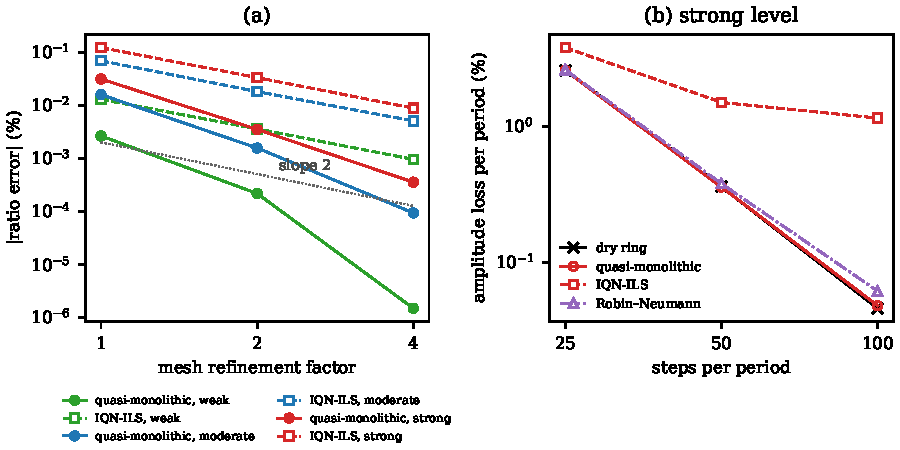
\includegraphics[width=0.85\textwidth]{figures/ringAddedMass-accuracy}
	\caption{Ring added-mass problem. (a) Error of the wet/dry frequency ratio against the mesh refinement factor at 100 steps per period, quasi-monolithic (filled) and IQN-ILS (open), for the three added-mass levels. (b) Amplitude loss per period against steps per period on the factor-2 mesh, strong level, with the dry ring.}
	\label{fig:ring_accuracy}
\end{figure}
% Data: paper-data/ring_monolithic_{mesh,runs}.csv (paper-fsi-verification ring-monolithic, ff150e4); script figures/scripts/ring_accuracy.py.

% Data: Mx 5400191 (a421f063d), paper-data/campaign/d/timing-ma on
% evidence/m-runs-d (timing_ma_summary.md); ratio errors from the timing
% runs with the dry frequencies of the same mesh and steps
% (paper-fsi-verification ring-monolithic, ringAddedMass_monolithic_runs.csv).
\begin{table}[htbp]
	\centering
	\caption{Ring added-mass problem, strong level ($\mu = 10.08$), factor-2 mesh, four periods, one process: iterations, cost and accuracy of the three couplings. Iterations: Newton iterations (quasi-monolithic) or coupling iterations (partitioned) per step. Time: median solver execution time of three repeats per step. Ratio error: error of the wet/dry frequency ratio against the exact value.}
	\label{tab:ring_cost}
	\setlength{\tabcolsep}{3pt}
	\begin{tabular}{lrrrrr}
		\toprule
		Coupling & Steps/period & Iterations/step & Time/step (s) & Ratio error (\%) & Loss/period (\%) \\
		\midrule
		Quasi-monolithic & 25 & 2.0 & 0.32 & $-0.0070$ & 2.57 \\
		 & 50 & 2.0 & 0.30 & $-0.0052$ & 0.36 \\
		 & 100 & 2.0 & 0.29 & $-0.0035$ & 0.048 \\
		IQN-ILS & 25 & 4.2 & 0.55 & $+0.126$ & 3.77 \\
		 & 50 & 5.1 & 0.61 & $+0.101$ & 1.50 \\
		 & 100 & 5.2 & 0.56 & $+0.033$ & 1.15 \\
		Robin--Neumann & 25 & 46.5 & 4.03 & $-0.0058$ & 2.59 \\
		 & 50 & 37.3 & 2.50 & $-0.0085$ & 0.38 \\
		 & 100 & 11.7 & 0.79 & $-0.0085$ & 0.062 \\
		\bottomrule
	\end{tabular}
\end{table}

At the strong level every step of the quasi-monolithic coupling converges in two Newton iterations, with 20--22 Krylov iterations per Newton iteration, and a step costs about half as much as an IQN-ILS step at every time step (Table~\ref{tab:ring_cost}).
IQN-ILS needs four to five coupling iterations per step and, at its coupling tolerance, leaves a ratio error of $0.03$--$0.13\%$ and an amplitude loss above that of the other two couplings; the quasi-monolithic and Robin--Neumann couplings agree with each other in both quantities.
Robin--Neumann reaches the same accuracy as the quasi-monolithic coupling, but its coupling iterations grow as the time step increases, from 12 per step at 100 steps per period to 47 at 25, so that it is 3 to 13 times as expensive and, unlike the other two, becomes more expensive per period as the time step grows.

Under mesh refinement at 100 steps per period, the ratio error of the quasi-monolithic coupling falls faster than second order at every added-mass level (observed orders 3.2--3.3 at the strong level, 3.3--4.1 at the moderate level and higher at the weak level), to below $4\times10^{-4}\%$ on the factor-4 mesh (Figure~\ref{fig:ring_accuracy}a): the wet and dry runs share the solid and temporal errors, which cancel in the ratio.
The IQN-ILS ratio error converges at order 1.8--1.9 and is 25 to 600 times larger on the factor-4 mesh.
The coupling adds no measurable damping: at the strong level the amplitude loss per period of the quasi-monolithic coupling equals that of the dry ring to within 0.004 percentage points at every time step (Figure~\ref{fig:ring_accuracy}b), so the loss is the numerical damping of BDF2 in the ring itself, which falls by a factor of 7--8 per halving of the time step; on all three meshes and levels at 100 steps per period the wet and dry losses differ by at most 0.08 percentage points, against 0.06 to 2.1 percentage points of additional loss for IQN-ILS.
Every quasi-monolithic step converges in two Newton iterations at every added-mass level and time step on the factor-2 mesh.
% Recorded before the tag (stale, for orientation only; ringAddedMass
% verification/README.md lines 319-371): 2.00 Newton iterations per step at
% every level and step; amplitude loss equal to the dry ring's.

%%--------------------------------------------------------------------------------------------------------------------%%
\subsection{Pulsatile compliant tube}\label{sec:womersley_m}
% TIME-SCHEME NOTE (Philip, 22 Oct 2026), for anyone adding results here:
% all transient results in this paper must use BDF2 (backward) for the fluid
% ddt(U) and the solid. The solids4foam tutorial default for this case is
% backward for the fluid ddt(U). Confirm and record the ddt schemes of every
% run (runs.csv); rerun any result computed with Euler, and say so here.
% Confirmed 31 Oct 2026: ddt(U) backward in every run (runs.csv of evidence/m-runs-a-rfix); solid default backward (tutorial *.monolithic).
%%--------------------------------------------------------------------------------------------------------------------%%
% Set-up: companion paper sectionBenchmarkSuite.tex "Pulsatile compliant tube";
% solids4foam 257b2e564 tutorials/fluidSolidInteraction/womersleyTube/
% verification/README.md section "Quasi-monolithic coupling" (lines 315-351).
% Monolithic solid: linearGeometryVelocity, conformal direct map.
% Driver: verification/Allverify --monolithic.

A harmonic pressure wave travelling along an axisymmetric thick-walled elastic tube combines added mass, viscous attenuation and a deforming wall, and its exact linear solution~\citetodo{companion verification paper} measures the error of the viscous interface traction, which the ring problem, with an effectively inviscid fluid, does not.

\paragraph{Set-up.}
The tube of the companion paper is used unchanged ($h/R = 0.1$, $L/R = 15$, Womersley number $5.01$, $\rho_s h/(\rho_f R) = 0.1$), with exact travelling-wave data at both ends and exact initial fields, on a wedge mesh.
Meshes are refined by factors 1, 2 and 4 at 200 steps per period, and 50 to 400 steps per period are used on the factor-2 mesh.
First Fourier coefficients over periods 5--6 are compared with the exact solution; the fluid and the solid both use BDF2, and the Newton tolerances are tightened to $10^{-8}$ (Krylov $10^{-6}$) so that the iterative error is negligible.
The partitioned runs of the companion paper need a flux-consistent treatment of the tube ends (the \texttt{pimpleFluid} option \texttt{fluxConsistentPatches}) to recover second order in time; the quasi-monolithic runs, with the end conditions of the tutorial's quasi-monolithic variant and no such option, converge at second order in time (Table~\ref{tab:womersley_m}).

\paragraph{Measured.}
Errors and observed orders in space and time of the velocity profile, the flow-rate amplitude and phase, the wall displacement amplitude and phase, the wave speed and the attenuation; Newton and Krylov iterations; and cost against IQN-ILS and Robin--Neumann on the factor-2 mesh at 100 steps per period.
The difference between the couplings is discussed in Section~\ref{sec:womersley_consistency}.

% Data: evidence/m-runs-a-rfix:paper-data/campaign/m-runs-a-rfix/qois.csv (build 1252bd2e5, R-fix);
% orders from successive differences of the values.
\begin{table}[htbp]
	\centering
	\caption{Pulsatile compliant tube, quasi-monolithic coupling (build \texttt{1252bd2e5}): observed orders in space (factors 1/2/4 at 200 steps per period) and time (factor-2 mesh), and the error on the factor-4 mesh at 200 steps per period. Errors are relative, except phases (rad).}
	\label{tab:womersley_m}
	\begin{tabular}{lrrrr}
		\toprule
		Quantity & Space & Time 50/100/200 & Time 100/200/400 & Error, factor 4 \\
		\midrule
		Velocity profile (max.) & 1.81 & --$^{a}$ & 1.91 & $9.6\times10^{-4}$ \\
		Flow-rate amplitude & 2.06 & 2.03 & 2.01 & $-3.4\times10^{-4}$ \\
		Flow-rate phase & 1.92 & 1.86 & 1.93 & $8.4\times10^{-5}$ \\
		Wall displacement amplitude & 1.98 & 1.96 & 1.99 & $-3.5\times10^{-4}$ \\
		Wall displacement phase & 1.46 & 2.14 & 2.07 & $-1.2\times10^{-3}$ \\
		Wave speed & 2.00 & 1.94 & 1.98 & $-6.0\times10^{-6}$ \\
		Attenuation & --$^{b}$ & 2.11 & 2.06 & $-1.9\times10^{-3}$ \\
		Pressure amplitude & 2.37 & --$^{a}$ & 1.88 & $1.5\times10^{-3}$ \\
		\bottomrule
	\end{tabular}

	\smallskip
	{\footnotesize $^{a}$ change between 100 and 200 steps per period below $2\times10^{-5}$, so no order is formed. $^{b}$ the error changes by less than $15\%$ between meshes and not monotonically.}
\end{table}

Every quantity converges at second order in time (observed orders 1.86--2.14, Table~\ref{tab:womersley_m}), and the flow rate, the wall displacement amplitude, the wave speed and the pressure converge at second order in space (1.92--2.37; the velocity profile at 1.81), with every quasi-monolithic step converging in two Newton iterations and 23--28 Krylov iterations per Newton iteration; the partitioned runs need 15--16 (IQN-ILS) and 11--18 (Robin--Neumann) coupling iterations per step at the strict test.
The wall displacement phase and the attenuation are the exceptions: their errors fall only from $2.4$ to $1.2\times10^{-3}\,\mathrm{rad}$ and from $0.23\%$ to $0.19\%$ between the factor-1 and factor-4 meshes, and about $1.2\times10^{-3}\,\mathrm{rad}$ and $0.15\%$ remain on the factor-2 mesh when the time step is extrapolated to zero.
Robin--Neumann shows the same phase and attenuation to within $5\times10^{-5}\,\mathrm{rad}$ and $3\times10^{-4}$ (Section~\ref{sec:womersley_consistency}), so this error belongs to what the two couplings share, not to the coupling; the partitioned study of the companion paper finds the same wall-phase order (1.40) and the same attenuation error ($-2\times10^{-3}$ on every mesh and time step), the latter at the accuracy limit of the linear theory used as the reference~\citetodo{companion verification paper}.
The timings of these runs were taken on a shared node and are not reported.

%%--------------------------------------------------------------------------------------------------------------------%%
\subsection{Effect of the interface treatment}\label{sec:interface_comparison}
%%--------------------------------------------------------------------------------------------------------------------%%
% Comparisons selected per Philip's decision (20 Oct 2026): only those that are
% an option on the tag and informative. Routes and run sets from audit A4
% (paper-data/a4_ablation_reproducibility.md, Sections 1 and 7).

Two ingredients of the interface treatment of Section~\ref{sec:interface_conditions} can be switched by an option and are examined here on the ring problem, whose exact solution attributes any change to the ingredient removed.

\paragraph{Interface pressure.}
The normal pressure gradient of Equation~\eqref{eqn:interface_pressure_gradient} is replaced by a zero normal gradient on the interface, with everything else unchanged, including the face extrapolation of the solid velocity.
% A4 Section 1: change the interface entry of 0/fluid/p.monolithic to
% zeroGradient; the coupler only warns (Coupler:2093-2112). Run the conformal
% arm of Allverify --study nonconformal, --levels moderate,strong.
The moderate and strong levels are run on mesh factors 1, 2 and 4 at 100 steps per period.

% Data: paper-data/ring_pressure_condition.csv (evidence/m-runs-a-rfix qois.csv, runs 1a and 1b, solids4foam 1252bd2e5);
% figure: figures/scripts/ring_pressure_condition.py.
\begin{figure}[htbp]
	\centering
	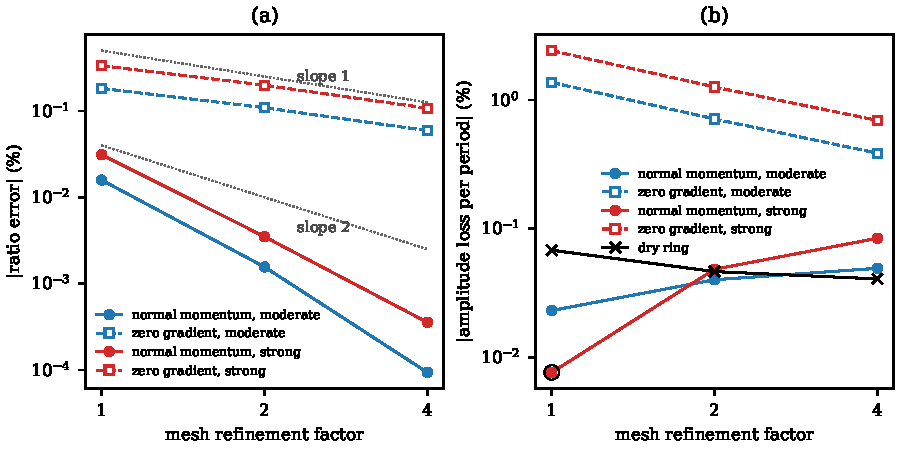
\includegraphics[width=\linewidth]{figures/ringAddedMass-pressure-condition.pdf}
	\caption{Ring added-mass problem, quasi-monolithic coupling at 100 steps per period: interface pressure from the normal momentum equation (filled) against a zero normal gradient (open), moderate and strong levels. (a) Magnitude of the relative error of the wet/dry frequency ratio and (b) magnitude of the amplitude loss per period against mesh refinement factor, with the dry ring in (b). The circled point is an amplitude growth of $0.008\%$ per period (strong level, factor 1). solids4foam \texttt{1252bd2e5}.}
	\label{fig:ring_pressure_condition}
\end{figure}

With a zero normal pressure gradient the ratio error converges at first order, with observed orders 0.74 and 0.88 at the moderate level and 0.75 and 0.89 at the strong level, and is 300 to 600 times larger on the factor-4 mesh than with the normal-momentum gradient ($0.059\%$ and $0.108\%$, against $9\times10^{-5}\%$ and $4\times10^{-4}\%$; Figure~\ref{fig:ring_pressure_condition}a).
The zero gradient also damps the coupled vibration: the amplitude loss per period exceeds that of the dry ring by $1.3$, $0.66$ and $0.34$ percentage points at the moderate level and by $2.3$, $1.2$ and $0.65$ at the strong level on the three meshes, halving with each refinement, whereas with the normal-momentum gradient the wet and dry losses differ by at most $0.08$ percentage points (Figure~\ref{fig:ring_pressure_condition}b).
A zero gradient is consistent only in the limit of a stationary interface; on a moving interface it omits the pressure gradient that accelerates the fluid with the wall, which is the added-mass effect itself; this is consistent with an error that grows with the added mass and falls at first order with the size of the cells adjacent to the interface.
The interface pressure treatment therefore controls the damping of the coupled vibration as well as its frequency.

\paragraph{Non-conformal transfer.}
The ring is computed with solid interface meshes coarser and finer than the fluid interface mesh, coupled through the AMI weights, once with interpolated traction and once with the conservative transfer of Equation~\eqref{eqn:conservative_transfer}.
% A4 Section 7: Allverify --study nonconformal (factors 1/2/4 x solid
% interface {conformal, coarser, finer} at 100 steps per period), once with
% conservativeTractionTransfer no and once yes, with
% interfaceFluxDiagnostics yes (logs rel_imbalance). RAM uses
% linearGeometryVelocity, so useUndeformedArea is not needed.
The total interface force transferred is logged on both sides of the interface at every step.

% Data: paper-data/ring_nonconformal.csv (MeluXina 5407040, a421f063d, interfaceFluxDiagnostics yes; ratios
% identical to the R-fix 1c runs at 1252bd2e5); figure: figures/scripts/ring_nonconformal.py.
% The code logs the force balance only, not the interface power.
\begin{figure}[htbp]
	\centering
	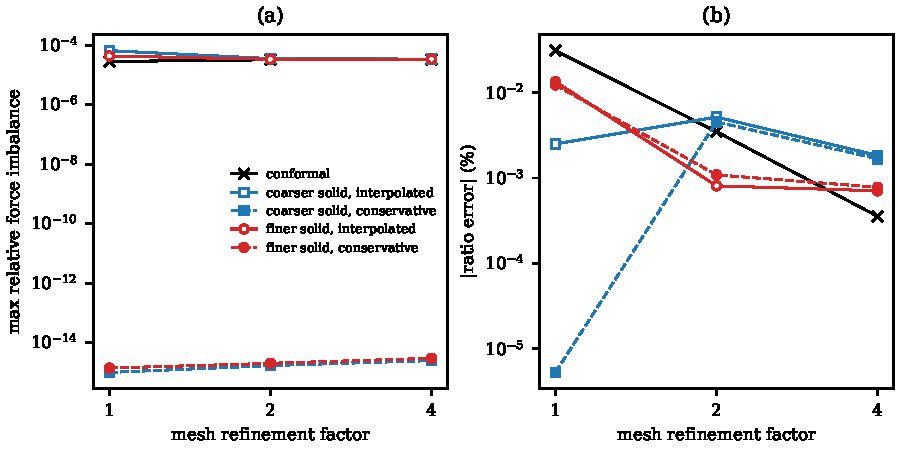
\includegraphics[width=\linewidth]{figures/ringAddedMass-nonconformal.pdf}
	\caption{Ring added-mass problem on non-conformal interfaces, quasi-monolithic coupling, strong level, 100 steps per period: (a) largest relative imbalance of the total interface force over the run and (b) magnitude of the relative error of the wet/dry frequency ratio against mesh refinement factor, for a conformal interface (direct map) and for solid interfaces with $32$ (coarser) and $72$ (finer) circumferential faces per mesh factor against $48$ on the fluid side, with interpolated (open) and conservative (filled) traction transfer. solids4foam \texttt{a421f063d}.}
	\label{fig:ring_nonconformal}
\end{figure}

With the conservative transfer the total force on the solid equals that of the fluid to round-off, with a relative imbalance below $3\times10^{-15}$ at every step, mesh and level (Figure~\ref{fig:ring_nonconformal}a).
With interpolated traction the imbalance is $3$--$9\times10^{-5}$ and does not decrease with refinement, but it is not an error of the transfer: on the factor-2 and factor-4 meshes it equals that of the conformal direct map to within $10\%$ ($2$--$3\times10^{-5}$ at the strong level, $5$--$8\times10^{-5}$ at the moderate level), which arises because the linear-geometry solid integrates the traction over its undeformed face areas while the fluid integrates over the deformed faces.
The frequency ratio is not affected by the choice of transfer at the reported precision: the interpolated and conservative results differ by at most $2.6\times10^{-5}$ relative on every mesh and level, and on the factor-4 mesh the ratio error on a non-conformal interface is $1.9\times10^{-5}$ or less, against $4\times10^{-6}$ or less on the conformal interface (Figure~\ref{fig:ring_nonconformal}b).

Two further ingredients were established during development and cannot be switched off in the released code, so their effect is quoted from the solids4foam commits that introduced them rather than rerun: removing a one-step lag of the interface force in the velocity solid reduced the amplitude loss per period of the ring at 100 steps per period from $2.0$, $10.6$ and $18.3\%$ to $0.17$, $0.71$ and $1.26\%$ (weak, moderate, strong), and evaluating the viscous traction as the momentum wall flux rather than from the deviatoric stress raised the observed spatial order of the blobInTreacle displacement, a stationary-wall case, from $1.4$ to $2.0$.
% Sources: ringAddedMass/verification/README.md "Defects found by this
% study" and commit messages dcbe04505 -> c008e8dd1 (force lag, both states
% with zeroGradient interface pressure); blobInTreacle/verification/README.md
% lines 203-208, states 0698d55cd -> dbfda65ba (traction only). A4 Sections
% 2 and 3a. Numbers recorded at those commits, not rerun from the tag.
% Decision (Philip, 31 Oct 2026): quoting these historical pairs is approved, and the
% stationary-wall qualification stays.
